% Options for packages loaded elsewhere
\PassOptionsToPackage{unicode}{hyperref}
\PassOptionsToPackage{hyphens}{url}
%
\documentclass[
]{article}
\usepackage{amsmath,amssymb}
\usepackage{iftex}
\ifPDFTeX
  \usepackage[T1]{fontenc}
  \usepackage[utf8]{inputenc}
  \usepackage{textcomp} % provide euro and other symbols
\else % if luatex or xetex
  \usepackage{unicode-math} % this also loads fontspec
  \defaultfontfeatures{Scale=MatchLowercase}
  \defaultfontfeatures[\rmfamily]{Ligatures=TeX,Scale=1}
\fi
\usepackage{lmodern}
\ifPDFTeX\else
  % xetex/luatex font selection
\fi
% Use upquote if available, for straight quotes in verbatim environments
\IfFileExists{upquote.sty}{\usepackage{upquote}}{}
\IfFileExists{microtype.sty}{% use microtype if available
  \usepackage[]{microtype}
  \UseMicrotypeSet[protrusion]{basicmath} % disable protrusion for tt fonts
}{}
\makeatletter
\@ifundefined{KOMAClassName}{% if non-KOMA class
  \IfFileExists{parskip.sty}{%
    \usepackage{parskip}
  }{% else
    \setlength{\parindent}{0pt}
    \setlength{\parskip}{6pt plus 2pt minus 1pt}}
}{% if KOMA class
  \KOMAoptions{parskip=half}}
\makeatother
\usepackage{xcolor}
\usepackage[margin=1in]{geometry}
\usepackage{graphicx}
\makeatletter
\def\maxwidth{\ifdim\Gin@nat@width>\linewidth\linewidth\else\Gin@nat@width\fi}
\def\maxheight{\ifdim\Gin@nat@height>\textheight\textheight\else\Gin@nat@height\fi}
\makeatother
% Scale images if necessary, so that they will not overflow the page
% margins by default, and it is still possible to overwrite the defaults
% using explicit options in \includegraphics[width, height, ...]{}
\setkeys{Gin}{width=\maxwidth,height=\maxheight,keepaspectratio}
% Set default figure placement to htbp
\makeatletter
\def\fps@figure{htbp}
\makeatother
\setlength{\emergencystretch}{3em} % prevent overfull lines
\providecommand{\tightlist}{%
  \setlength{\itemsep}{0pt}\setlength{\parskip}{0pt}}
\setcounter{secnumdepth}{5}
\newlength{\cslhangindent}
\setlength{\cslhangindent}{1.5em}
\newlength{\csllabelwidth}
\setlength{\csllabelwidth}{3em}
\newlength{\cslentryspacingunit} % times entry-spacing
\setlength{\cslentryspacingunit}{\parskip}
\newenvironment{CSLReferences}[2] % #1 hanging-ident, #2 entry spacing
 {% don't indent paragraphs
  \setlength{\parindent}{0pt}
  % turn on hanging indent if param 1 is 1
  \ifodd #1
  \let\oldpar\par
  \def\par{\hangindent=\cslhangindent\oldpar}
  \fi
  % set entry spacing
  \setlength{\parskip}{#2\cslentryspacingunit}
 }%
 {}
\usepackage{calc}
\newcommand{\CSLBlock}[1]{#1\hfill\break}
\newcommand{\CSLLeftMargin}[1]{\parbox[t]{\csllabelwidth}{#1}}
\newcommand{\CSLRightInline}[1]{\parbox[t]{\linewidth - \csllabelwidth}{#1}\break}
\newcommand{\CSLIndent}[1]{\hspace{\cslhangindent}#1}
\usepackage{setspace}
\usepackage{float}
\floatplacement{figure}{H}
\ifLuaTeX
  \usepackage{selnolig}  % disable illegal ligatures
\fi
\IfFileExists{bookmark.sty}{\usepackage{bookmark}}{\usepackage{hyperref}}
\IfFileExists{xurl.sty}{\usepackage{xurl}}{} % add URL line breaks if available
\urlstyle{same}
\hypersetup{
  pdfauthor={Daniel Bonfil},
  hidelinks,
  pdfcreator={LaTeX via pandoc}}

\title{\hfill\break
\hfill\break
Presidential Success in Mexico and the US Economy:\\
Remittances and Misattribution of Responsibility\\
\strut \\}
\usepackage{etoolbox}
\makeatletter
\providecommand{\subtitle}[1]{% add subtitle to \maketitle
  \apptocmd{\@title}{\par {\large #1 \par}}{}{}
}
\makeatother
\subtitle{\hfill\break
\hfill\break
FGV EBAPE\\
\strut \\
\strut \\
Comparative Political Economy\\
(Daniela Campello)\\
\strut \\}
\author{Daniel Bonfil}
\date{2024-01-05}

\begin{document}
\maketitle

{
\setcounter{tocdepth}{2}
\tableofcontents
}
\newpage
\doublespacing

\hypertarget{abstract}{%
\subsection{Abstract}\label{abstract}}

While economic factors beyond incumbents' control, such as oil prices
and international interest rates, often dictate presidential success in
Latin America, the case of Mexico presents a puzzle. Research by
Campello \& Zucco (2016) shows how Low Savings Commodity Exporting
(LSCE) Latin American countries tie presidents' fate to external
economic swings, but in Mexico, the link appears weaker. This suggests
that other factors influence Mexican presidential success, potentially
including the impact of the US economy. I propose that Mexico's unique
characteristics, shaped by long-term migration and economic ties to the
US, make it less sensitive to traditional exogenous shocks but more
susceptible to those specific to the conditions of the US economy. I
focus on this relationship and the mechanism of misattribution of
responsibility, which occurs when citizens mistakenly assign economic
outcomes to presidential performance, regardless of its true cause. I
contend that citizen perceptions towards positive economic conditions,
largely determined by specific fluctuations in the US economy such as
remittance flows and strong employment in the construction sector,
significantly impact Mexican presidential approval, potentially
advancing misattribution. This research aims to better characterize the
factors beyond commodity prices and interest rates that influence
Mexican presidential success.

\hypertarget{introduction}{%
\subsection{Introduction}\label{introduction}}

Mexico is both part of Latin American countries due to its Spanish
heritage and of North America because of its geography. The presence of
Mexican culture is widely present in Central and South America however,
its economic dynamics differ from that of its Latin American peers.
Decades of integration with its two northern Anglo American neighbors,
mainly through migration and economic agreements, have come to shape the
country characteristics that distinguish Mexico within both regions.

The issue of misattribution of responsibility occurs when voters
attribute economic conditions to incumbents even when those conditions
are determined by factors beyond governmental control (Campello \&
Zucco, 2022). Campello \& Zucco (2020) claim that exposure to exogenous
shocks, strongly associated with dependence on commodities and
variations in trade, is a fundamental structural difference between
developed and developing economies. They argue that countries highly
exposed to volatile exogenous conditions face more challenges in
identifying the competence of governments based on the economy.

For a large subset of Latin American countries, presidential popularity
and reelection prospects strongly depend on factors exogenous to
presidents' policy choices such as commodity prices and international
interest rates. Campello \& Zucco (2016) demonstrate that international
economic conditions affecting LSCE countries like Brazil, do not impact
Mexico in the same way. Brazil stands out as a commodity-exporting
nation highly reliant on international capital flows, while Mexico
distinguishes itself as one of the least commodity-dependent countries
in Latin America. Mexico's unique position is attributed to its close
ties with the US consumer market, making it more receptive to financial
capital during favorable economic conditions in the United States. This
is particularly evident during periods of rising interest rates,
indicative of a robust economy.

This observation is particularly compelling, it signals that other
external factors beyond international interest rates and commodity
prices influence presidential popularity in Mexico. I contend that
country characteristics resulting from long-term migration and economic
evolution make Mexico less vulnerable to interest rate shocks and
commodity prices but also to other factors that result from exogenous
shocks rooted in the conditions of the US economy, specifically
remittance flows (Germano, 2013) and strong employment in the
construction sector (Cañas \& Pranger, 2023).

The impact of migration on Mexico has been substantial, driven by
diverse needs but ultimately converging on the aspiration for improved
living conditions. Historically employed in the US, Mexican migrant
workers shifted sectors over the years, with recent concentrations in
Construction and Hospitality and Leisure (Cañas \& Pranger, 2023;
Serrano et al., 2022). As of 2022, Mexico became the world's
second-highest receiver of remittances, constituting 4.5\% of its GDP,
following only India (Serrano et al., 2022). In terms of trade, Mexico
surpassed Canada as the top US trading partner in 2023 and China
becoming the primary manufacturing partner in 2022, driven by
post-pandemic nearshoring dynamics and technological advancements in the
traditional Mexican ``Maquila.'' Economic reforms and 13 free trade
agreements, and particularly the USMCA, further bolstered Mexico's trade
position, attracting substantial foreign direct investment and
establishing it as a long-term operational hub (Buendía, 1996; Cameron
\& Wise, 2004; Torres, 2023).

Despite trade liberalization efforts and enhanced competitiveness,
strong labor demand in the US continues to attract migrants, in 2021 a
total of 11.9 million Mexican migrants lived in the US (Serrano et al.,
2022). Endogeneity concerns should be considered since migration could
be a consequence of poor long-term policymaking, forcing Mexicans to
seek job opportunities elsewhere. However, underlying conditions in the
US would determine demand for labor and trade, resulting in exogenous
shocks. Beyond the benefits and consequences of trade, remittances, a
historically increasing financial flow are sent by migrant workers to
support Mexican households (Doyle, 2015; Doyle \& López García, 2021).
Counterintuitively, remittances are commonly attributed as a
presidential accomplishment regardless of the fact that these transfers
originate from conditions in the US and migrant workers.

This matters because the positive perception of the increasing flow of
remittances might result in misattribution of responsibility for an
accomplishment beyond presidential policymaking. Hence, in order to
amplify the fitting power of the model introduced by Campello \& Zucco
(2016) and drawing inspiration from Bravo (2012), Tertytchnaya et al.
(2018), and Doyle \& López García (2021), I hypothesize that exogenous
shocks resulting from i) remittances flows and ii) strong labor demand
in the US construction sector, could help better characterize the
exogenous shocks conditions and whether or not they have an effect on
presidential approval for the case of Mexico.

The remainder of the article is structured as follows: Section (3)
introduces notions of assignment of responsibility, economic voting, and
presidential success. Alongside, I explain the relationship between
remittances, employment in the construction sector, and presidential
approval. In Section (4), I discuss relevant factors about Central and
Latin America, as well as oil and security dynamics in Mexico. Section
(5) describes the experimental design and data, followed by the
hypotheses, and expected results in Section (6). Finally, I portray the
implications and limitations of the proposed study in Section (7).

\hypertarget{literature-review}{%
\subsection{Literature Review}\label{literature-review}}

The relationship between remittances and economic growth has been a
topic of debate suggesting that remittances act as a vital international
risk-sharing mechanism (Yang \& Choi, 2007), of being largely outside
the control of governments in migrant home countries (Germano, 2013), to
color economic assessments and dampen the political effects of a variety
of economic shocks (Bravo, 2012), and considered a political
manifestation of economic dependency (Wibbels, 2006). Doyle (2015) and
Tertytchnaya et al. (2018) contribute to the literature by examining the
underexplored relationship between fluctuations in remitted income and
incumbent evaluations. Their study reinforces assumptions about voters'
overestimated ability to disentangle competence from exogenous shocks,
particularly in low-information, developing country contexts (Campello
\& Zucco, 2020).

In developing democracies, support for incumbents is often influenced by
economic and political developments abroad, such as commodity price
shocks (Monteiro \& Ferraz, 2012). Campello \& Zucco (2016) use the Good
Economic Times (GET) Index\footnote{The GET Index, devised to gauge the
  economic environment faced by Latin American countries, combines
  monthly values of US 10 Year Treasury Constant Maturity Rate and
  UNCTAD's ``Free Market Commodity Prices'' Index. Through principal
  components decomposition, it condenses these variables into a
  one-dimensional indicator on a unitless normalized scale. Higher GET
  values signify favorable economic conditions, while lower values
  indicate challenging times for the region. The authors justify this
  simplified approach for its ability to capture variations in
  international conditions, considering both commodity prices and US
  interest rates. The index is employed in the study to examine its
  impact on domestic economic indicators and presidential popularity,
  particularly distinguishing within 18 Latin American countries, 10 in
  the LSCE sample and 8 in the comparison group.} based on commodity
prices and US interest rates to explain that voters in LSCE countries in
Latin America misattribute responsibility for economic outcomes to
incumbents. This misattribution, driven by exogenous shocks, has
implications for the efficacy of the economic vote as a mechanism of
accountability.

Doyle (2015) delves into the relationship between remittances and social
spending in developing economies by exploring the impact of remittances
on income levels, economic security, and the subsequent implications for
social welfare transfers. Findings by Doyle (2015) are in line with Yang
\& Choi (2007), reinforcing the perspective of how remittances increase
significantly in response to macroeconomic shocks, acting as a
stabilizing force in times of economic uncertainty. Doyle (2015) posits
that remittances serve as an insurance and compensation mechanism,
contributing to the stability of domestic economies and that such
compensation function is further highlighted by the evidence that
remittances reduce household income volatility.

Similarly, Tertytchnaya et al. (2018) examine the impact of fluctuations
in remitted income on support for incumbents in remittance-receiving
countries in Central Eastern Europe, the Caucasus, and Central Asia. The
authors contend that remittance recipients, by relying on their
pocketbooks to assess government performance, may be attributing
economic developments abroad to the actions of incumbents at home. They
show that changes in remittances influence economic assessments and
incumbent approval, with increased remittance inflows leading to higher
economic evaluations and incumbent approval, while declines result in
punishment for incumbents.

Findings by Doyle (2015) and Tertytchnaya et al. (2018) challenge
traditional notions of economic voting (Fiorina, 1981; Kramer, 1971) and
competence misattribution in developed countries (Stevenson \& Duch,
2008), while reinforcing those of developing countries (Campello \&
Zucco, 2022). Economic voting can promote accountability, yet this does
not happen as voters reward or punish incumbents for economic outcomes
beyond their control, which is also known as misattribution of
responsibility. The authors support claims by Campello \& Zucco (2020)
stating that economic outcomes and assessments, even if largely driven
by exogenous factors, may be the only signal or source of information
about incumbent competence that voters have, yet for democratic
accountability to work properly, voters should punish or reward
incumbents based on outcomes for which they are inherently responsible
(Kayser \& Peress, 2012).

As Campello \& Zucco (2016) show, LSCE countries particularly dependent
on oil prices and international interest rates evaluate presidents based
on the positive or negative state of the economy, regardless of their
direct responsibility. However, the magnitude of exogenous factors
varies significantly among countries and regions. When Campello \& Zucco
(2016) evaluate the predictive power of the GET Index results show a
strong covariance between GET and presidential popularity in Brazil (R²
= 0.63) but a weak one in Mexico (R² = 0.12). Moreover, when comparing a
model with only the GET Index to a model with several domestic economic
variables, the GET model performs almost as well in predicting
popularity in Brazil but a null effect for Mexico. This finding leads me
to believe that country characteristics resulting from long-term
migration and economic integration make Mexico vulnerable to exogenous
factors of the US economy, specifically remittance flows (Germano, 2013)
and strong employment in the construction sector (Cañas \& Pranger,
2023).

The human trend of migration has had considerable effects in Mexico.
Migration originates from multiple sources of needs, yet they all
ultimately converge with the desire for better living conditions.
Mexican migrant workers have been historically employed in the US,
during the 2000's they worked mainly in the Commerce (23.6\%) and
Manufacturing (22.5\%) sectors, while more recently they are
concentrated in the Construction (19.5\%) and Hospitality and Leisure
(13.8\%) sectors (Cañas \& Pranger, 2023; Serrano et al., 2022). As of
2022, Mexico became the second-highest receiver of remittances in the
world, only behind India (\$55.9 and \$98.2 US billions, respectively)
but, this amount represents 4.5\% of the Mexican GDP while 2.9\% in the
case of India (Serrano et al., 2022).

With respect to trade, as of 2023, Mexico became the US top trading
partner surpassing Canada, while in 2022 it became its first
manufacturing partner surpassing China (Torres, 2023). Although this
shift accelerated due to post-pandemic nearshoring dynamics in the US,
such increased demand is only natural due to technological advances
allowing for the expansion and evolution of the traditional Mexican
``Maquila'' into a multifaceted trade hub. Moreover, this is also a
result of sound economic reforms and 13 free trade agreements with 50
countries, particularly those under the scope of the USMCA, which was
reformed in 2020 from the originally signed NAFTA in 1991 (Buendía,
1996; Cameron \& Wise, 2004). The rule of law conditions that emanated
from the trust relationship between Canada, US, and Mexico have enhanced
its appeal for larger flows of FDI that tend to establish operations for
longer time periods as opposed to shorter term investments that are most
prone to capital-flight dynamics (Campello, 2015).

Remittances are considered an exogenous and countercyclical capital flow
providing a unique opportunity to test misattribution of responsibility,
economic voting, and presidential success in Mexico. Germano (2013) and
Tertytchnaya et al. (2018) position remittances as exogenous capital
flows, largely beyond the control of governments in migrant home
countries. Cañas \& Pranger (2023) underscore the critical role of US
labor market conditions, particularly in the construction sector, in
driving the growth of remittances. They highlight the countercyclical
nature of remittances, which increase during economic downturns and
emphasize the intricate link between economic conditions in the host
country and remittance flows. The direct impact of remittances on
household income, coupled with their largely uncontrollable nature by
incumbent governments, makes them an excellent identification strategy
to examine how individuals attribute responsibility for exogenous
economic shocks.

\hypertarget{discussion}{%
\subsection{Discussion}\label{discussion}}

Campello \& Zucco (2016) explore presidential success and popularity
with the GET Index that display robust significant effects on
presidential reelection probabilities in LSCE countries, particularly
during favorable international economic conditions. Despite this,
authors acknowledge the challenges in predicting presidential elections,
emphasizing that most empirical work on economic voting is better at
predicting popularity than actual voting behavior. Tertytchnaya et al.
(2018) underscore the fragile equilibrium remittances can create,
influencing accountability mechanisms and governance dynamics in
remittance-dependent economies. Misattribution, whether rational or not,
poses normative challenges for democratic accountability, urging a
reconsideration of traditional economic voting models in the context of
exogenous shocks and remittance dependency.

\begin{figure}
\hypertarget{fig:label}{%
\centering
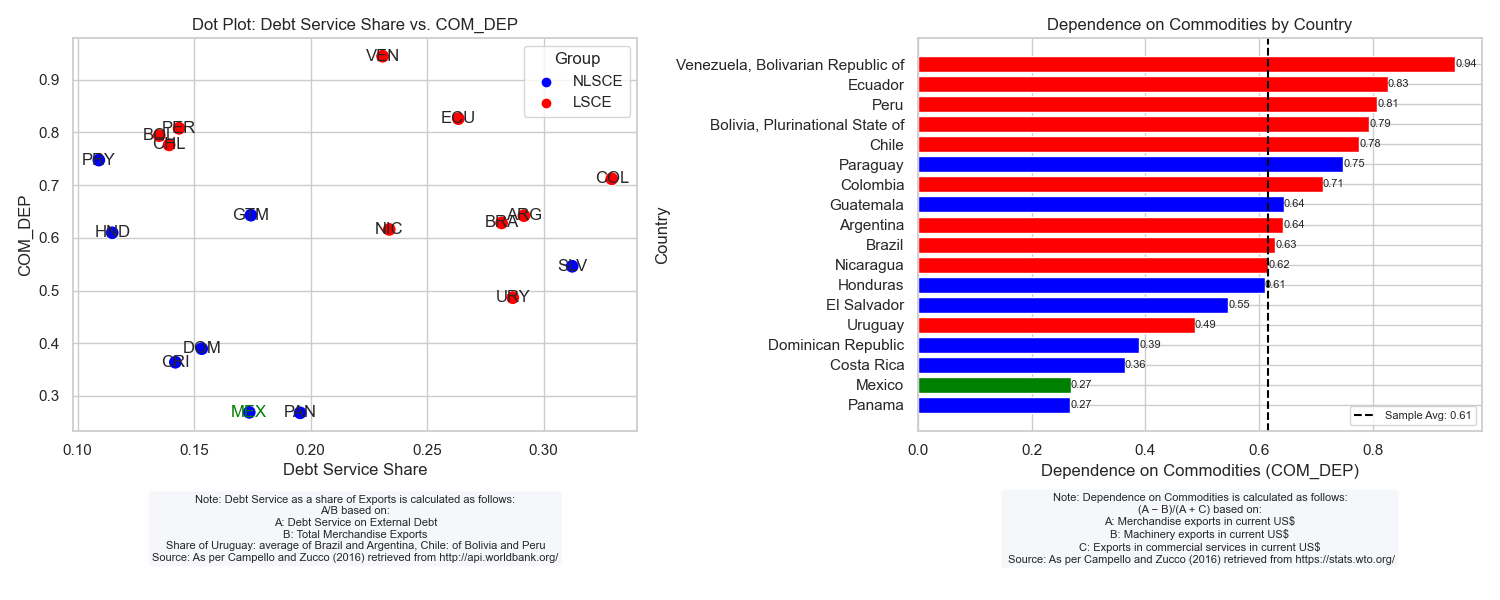
\includegraphics[width=1\textwidth,height=1\textheight]{com_debt_latam.png}
\caption{Debt Service Share and Commodity Dependence}\label{fig:label}
}
\end{figure}

The classification of countries into the LSCE category, consider most
South American countries and Nicaragua, which contrasts sharply with the
stance of Central American countries, Mexico and Paraguay, which
generally exhibit lower dependence on commodity exports. To quantify
this dependence, in Figure 1, I use data from the World Bank (WB) and
World Trade Organization (WTO) to compute the Debt Service as Share of
Exports and Dependence on Commodities, as outlined by Campello \& Zucco
(2016). The distinction in commodity dependence becomes crucial when
considering the economic vulnerabilities of countries in the region.
Nations heavily reliant on commodity exports often find themselves as
price takers in international trade markets, exposing them to the
cyclicality of prices and leading to significant fluctuations in export
earnings. During periods of high commodity prices, these countries
experience economic prosperity and increased export revenues.
Conversely, as prices decline, they face economic hardships.

\hypertarget{remittances-in-central-and-latin-america}{%
\subsubsection{Remittances in Central and Latin
America}\label{remittances-in-central-and-latin-america}}

Franzoni (2008) points out that countries with limited capacity to
establish large social programs experience higher migration and greater
remittance inflows, I compare latest and historical remittances as share
of GDP in the same Latin American Countries and the top 10
remittance-receiving countries in Figure 2 and 3 below. In the context
of small Central American states, where remittance inflows are
substantial, social security and welfare spending tend to be low and
favor the upper-income quintiles . For example, Ahmed (2017) describes
the dual impact of remittances in the Dominican Republic---eroding
clientelist linkages while, simultaneously, increasing support for the
incumbent due to positive economic perceptions among recipients.

\begin{figure}
\hypertarget{fig:label}{%
\centering
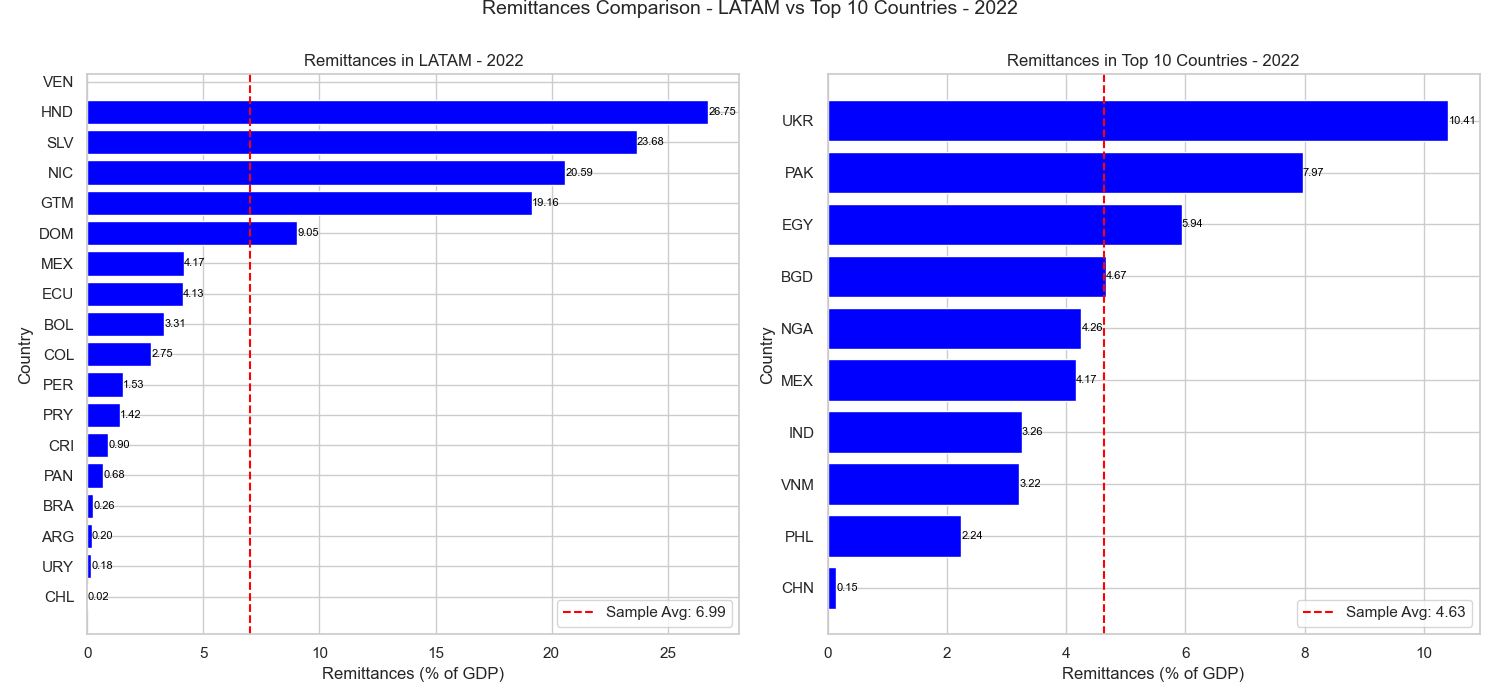
\includegraphics[width=1\textwidth,height=1\textheight]{rem22_lat_top.png}
\caption{Remittance as \% of GDP 2022}\label{fig:label}
}
\end{figure}

\begin{figure}
\hypertarget{fig:label}{%
\centering
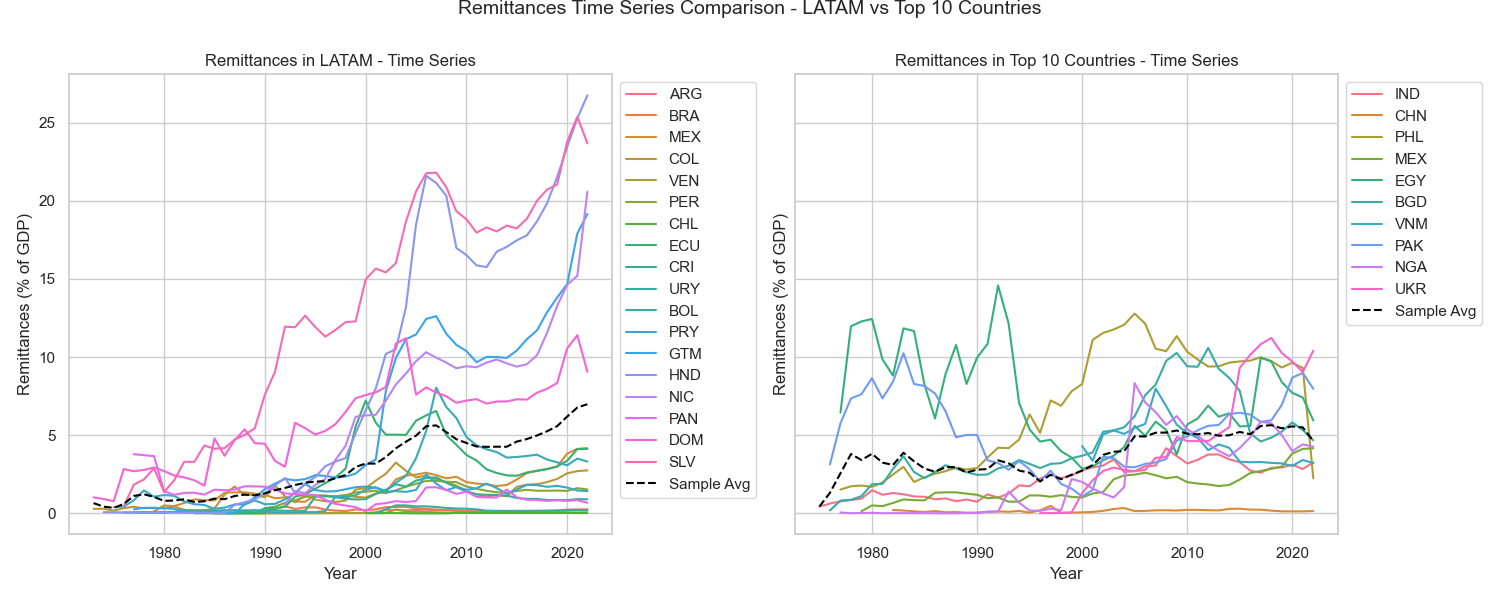
\includegraphics[width=1\textwidth,height=1\textheight]{remhist_lat_top.png}
\caption{Remittance as \% of GDP: Historical}\label{fig:label}
}
\end{figure}

Doyle (2015) uses the CEPALSTAT\footnote{Comisión Económica para América
  Latina y el Caribe (CEPAL)} database from 2014 to highlight that since
the 1990s, countries like Argentina, Brazil, and Mexico have witnessed
increased social transfers, while others like Bolivia, El Salvador, and
Peru experienced contractions or stagnation despite a global commodity
boom and left-leaning executives in power. The author suggests that
while remittances aren't the sole explanation, they contribute to the
unexplained heterogeneity of welfare regimes across the region,
particularly in countries with high levels of inequality and economic
insecurity (Doyle, 2015). The change in remittances as a share of GDP in
the same Latin American countries for 1, 5, and 10 years can be seen in
Figure 4, while that of the top remittance-receiving countries is
depicted in Figure 5.''

\begin{figure}
\hypertarget{fig:label}{%
\centering
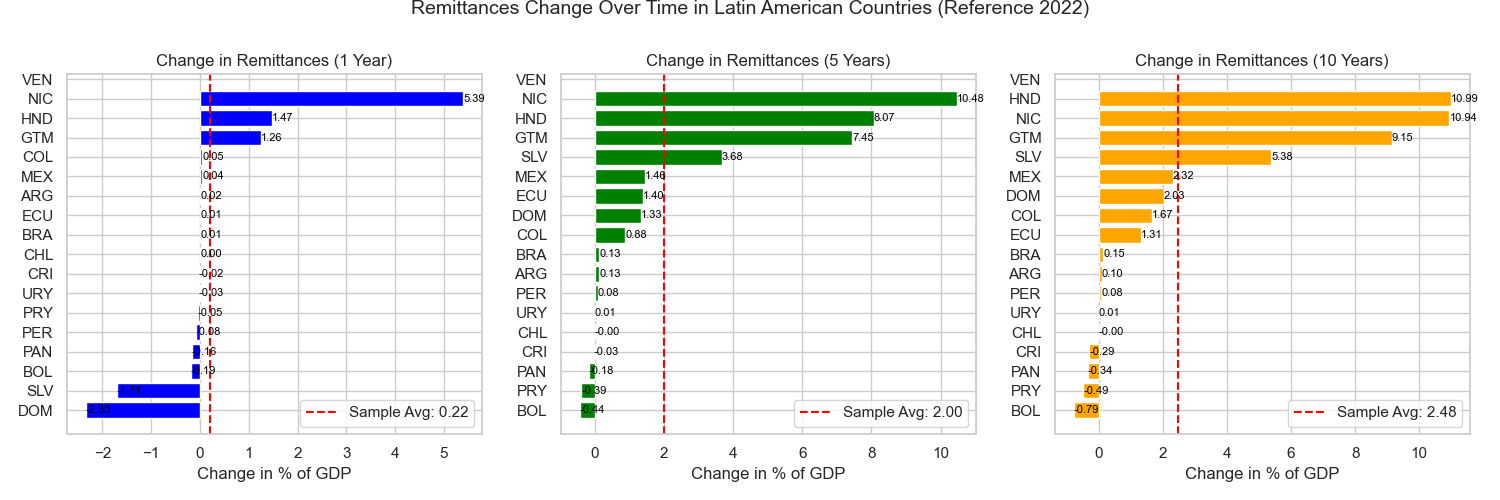
\includegraphics[width=1\textwidth,height=1\textheight]{remlat_chg.png}
\caption{Remittance \% Change Latam}\label{fig:label}
}
\end{figure}

\begin{figure}
\hypertarget{fig:label}{%
\centering
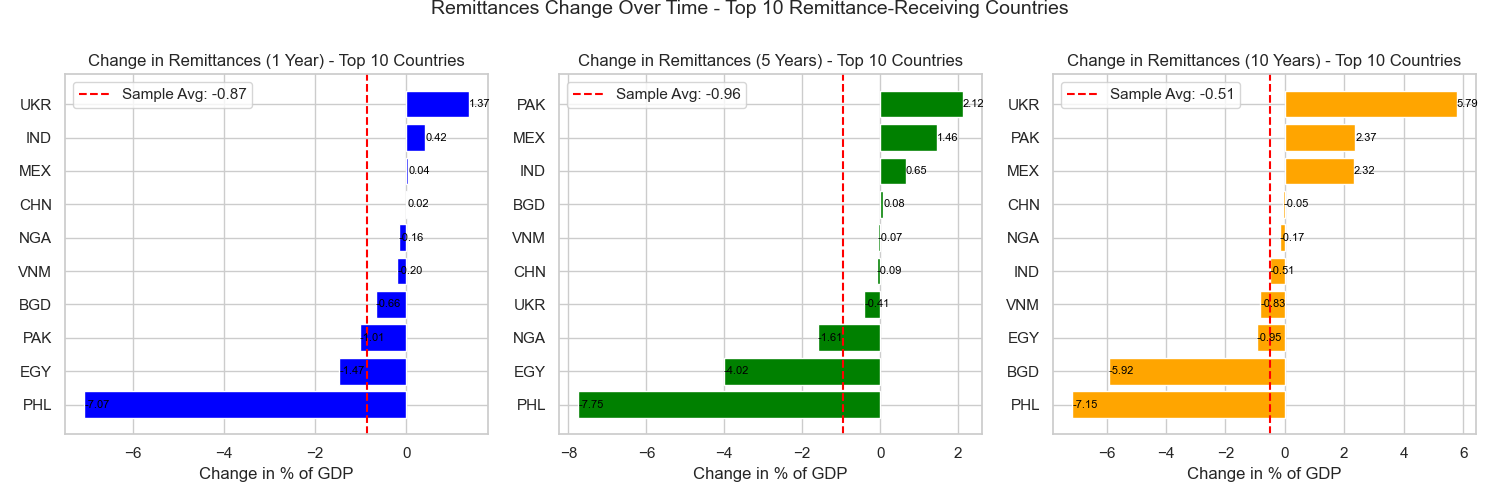
\includegraphics[width=1\textwidth,height=1\textheight]{remtop_chg.png}
\caption{Remittance \% Change Top Receving}\label{fig:label}
}
\end{figure}

Aparicio \& Meseguer (2012) demonstrate in Mexico that elected officials
strategically use remittances for political purposes, emphasizing the
potential misattribution of remittances. Doyle (2015) further elucidates
this argument by suggesting that this misattribution, particularly in
developing democracies, alters individual preferences towards
redistribution and taxation, potentially resulting in reduced social
welfare transfers being diverted towards patronage.

Ahmed (2017) argues that remittances act as unearned foreign income for
governments in autocracies, leading to reduced welfare spending. Doyle
(2015) extends this argument to democratic states, suggesting that
remittances, even in democracies, result in reduced social welfare
transfers, emphasizing the bottom-up causal mechanism where remittances
alter individual preferences towards redistribution and taxation.

\hypertarget{insecurity-and-crime}{%
\subsubsection{Insecurity and Crime}\label{insecurity-and-crime}}

It is tempting to study presidential approval with variables like
perceptions of security and crime, scholars like Romero et al. (2016)
and Doyle \& López García (2021) have argued that these predictors have
a weight in presidential success in Mexico, even more so than economic
performance. However, the foundations of these variables are more
endogenously-related given the state's responsibility for order and
governance. While one could make a case that insecurity could arise from
increased competition between Drug Trafficking Organizations (DTOs) on a
feud to protect or increase their share of the narcotics demand in the
US market, it could be more challenging to say that crime would be
exogenously-driven by factors in the US. It is precisely the exogenous
and countercyclical characteristics of remittances that allows for the
exploration of misattribution of responsibility.

Romero et al. (2016) and Doyle \& López García (2021) focus on the
influence of remittances on public security perceptions, personal
safety, and presidential approval. Contrary to the economic vote
hypothesis, they propose that remittances in Mexico impact approval
through enhanced security perceptions, given the nation's high crime
rates. Specifically, Romero et al. (2016) show that remittance
recipients report higher perceived safety and better national security
evaluations. Doyle \& López García (2021) reinforce such findings using
individual data from Mexico spanning six waves of the LAPOP\footnote{Americas
  Barometer Surveys 2004-2017. Pittsburgh: Vanderbilt University} public
opinion survey 2006--2017. Moreover, they employ causal mediation
analysis, revealing that nearly a quarter of the effect of remittances
on sociotropic security evaluations is mediated through improved
perceptions of personal safety.

Comparing these studies, both converge on the significance of security
in shaping presidential approval. However, they differ in their
emphasis, Romero et al. (2016) underscore the importance of symbolic
actions and a strong presidential stance on security, while Doyle \&
López García (2021) highlight the role of remittances in shaping
security perceptions. The studies diverge in their approach to economic
considerations, Romero et al. (2016) suggest citizens prioritize
security over economic concerns during security crises. In contrast,
Doyle \& López García (2021) argue that remittances, by alleviating
economic pressures associated with crime, contribute to improved
security evaluations and, consequently, presidential approval.

\hypertarget{oil-dependence-paradox}{%
\subsubsection{Oil-dependence Paradox}\label{oil-dependence-paradox}}

Mexico stands out as one of the world's largest crude oil exporters
ranking 12th globally, boasting extensive reserves enriched with
abundant heavy crude deposits. Pemex, the state-owned oil company, has
played a pivotal role in driving the country's oil export market,
shipping millions of barrels daily, predominantly to the United States
(Rodríguez, 2023). These crude oil exports significantly contribute to
Mexico's economic development, generating substantial revenue for the
government. However, a contradiction emerges as Mexico, despite being an
oil-producing nation, finds itself heavily reliant on the United States
for refined petroleum products, particularly gasoline.

The paradox is elucidated by Mexico's insufficient domestic refining
capacity, which lags behind its crude oil production. The country's
refineries often grapple with outdated infrastructure, requiring
substantial upgrades to efficiently process heavy crude into gasoline
and other refined products. Consequently, Mexico turns to importing
gasoline, with the United States emerging as a major supplier. The
decision to import gasoline is not merely driven by necessity but also
by cost considerations and expediency. Importing gasoline, particularly
from the US, proves to be a more economical and swift solution than
investing in extensive domestic refining upgrades.

Compared to the dependence of oil exporters in South America,
asseverations by Campello \& Zucco (2016) appear logical, yet on closer
inspection Mexico's position in the global oil market appears a two-fold
dependence, exporting crude while concurrently relying on foreign
sources for refined products. The latest Pemex third quarter report for
2023 reveals that Mexico imported 1.84 billion barrels of refined
products, primarily gasoline and diesel, while domestic refining
produced only 649 million barrels (Rodríguez, 2023). This stark contrast
highlights that over 70\% of Mexico's gasoline consumption is met
through imports, emphasizing the nation's significant dependence on
external suppliers. Because of this, I contend that the original GET
Index can be enhanced by including remittances flows, hopefully
achieving a better characterization of the index for the Mexican case.

\hypertarget{research-design-and-data}{%
\subsection{Research Design and Data}\label{research-design-and-data}}

For the dependent variable, presidential approval, I will follow Doyle
\& López García (2021), using individual data from Mexico obtained from
the LAPOP public opinion survey. This will enable me to explore the
relationship between the flow of remittances and approval for the
president. As for the predictors, first, I will replicate the original
GET Index by Campello \& Zucco (2016), which combines monthly values of
the US 10 Year Treasury Constant Maturity Rate and UNCTAD's `Free Market
Commodity Prices' Index.

\begin{itemize}
\tightlist
\item
  Second, I will create a database with:

  \begin{itemize}
  \tightlist
  \item
    Historic remittance flows of Mexico. Additionally, I will explore
    the values of Latin American countries and the Top 10
    remittance-receiving countries.
  \item
    Monthly construction employment from the Bureau of Labor Statistics
    payroll survey and median hourly nominal construction sector
    12-month wage growth from the Federal Reserve Bank of Atlanta's wage
    growth tracker. (See Annex) {[}\textbf{TBD: Leisure and Hospitality,
    the second sector employing Mexican migrants could be retrieved from
    the same source}{]}
  \item
    Alternatively, I will use either the FHFA (Federal Housing Finance
    Agency) House Price Index measures month over month changes in
    average prices of single-family houses with mortgages guaranteed by
    Fannie Mae and Freddie Mac. (See Annex)
  \item
    Or the DJUSRE index is designed to track the performance of real
    estate investment trusts (REIT) and other companies that invest
    directly or indirectly in real estate through development,
    management, or ownership, including property agencies. (See Annex)
  \end{itemize}
\item
  Finally, I will attempt to create an updated version of the GET Index
  that accounts for exogenous factors that attain the Mexican economy.
  By using the baseline model with commodities and interest rates, I
  will test the changes in presidential approval as I introduce
  remittance flows and construction statistics. Hopefully it can better
  characterize the variations in the economy that are relevant for
  presidential success and eventually election prospects.
\end{itemize}

\hypertarget{hypotheses-and-expected-results}{%
\subsection{Hypotheses and Expected
Results}\label{hypotheses-and-expected-results}}

\begin{itemize}
\tightlist
\item
  Hypotheses:

  \begin{itemize}
  \tightlist
  \item
    H1: Increases in remittance flows from the US positively influence
    presidential approval ratings in Mexico.
  \item
    H2: Strong employment in the US construction sector positively
    influences presidential approval ratings in Mexico.
  \item
    H3: Remittance flows and employment in the US construction sector
    will have a stronger correlation with presidential approval in
    Mexico compared to the influence of commodity prices and
    international interest rates.
  \end{itemize}
\item
  Expected Results:

  \begin{itemize}
  \tightlist
  \item
    E1: We expect to find a positive correlation between remittance
    flows and presidential approval ratings in Mexico. This means that
    as remittance flows increase, we would expect to see an increase in
    the percentage of citizens who approve of the president's
    performance.
  \item
    E2: We expect to find a positive correlation between strong
    employment in the US construction sector and presidential approval
    ratings in Mexico. This means that when US construction is booming
    and demand for Mexican labor is high, we would expect to see an
    increase in presidential approval.
  \item
    E3: Economic factors such as commodity prices and international
    interest rates have a weaker correlation with presidential approval
    in Mexico compared to the influence of remittance flows and
    employment in the US construction sector.
  \end{itemize}
\end{itemize}

\hypertarget{implications-and-limitations}{%
\subsection{Implications and
Limitations}\label{implications-and-limitations}}

Implications This research holds several implications that contribute to
a nuanced understanding of exogenous the factors influencing
presidential success and misattribution of responsibility in Mexico.
First and foremost, the identification of positive correlations between
increased remittance flows and higher levels of presidential approval,
as well as the influence of strong employment in the US construction
sector, underscores the significance of US-related factors in shaping
Mexican public opinion. By acknowledging the impact of remittances and
the US labor market on citizens' perceptions, the study can contribute
to the literature on misattribution of responsibility highlighting the
intricacies of public opinion formation in Mexico.

Citizens' tendency to attribute economic outcomes to the incumbent, even
when driven by external factors, underscores the need for a nuanced
approach to understanding voter behavior. This insight may pave the way
for further research into the psychological dimensions of political
decision-making, offering a deeper understanding of how citizens
interpret and assign credit or blame for economic conditions.
Ultimately, the implications of this research extend beyond the Mexican
context, providing valuable insights for scholars and policymakers
dealing with similar dynamics in other countries of Central and South
America with close economic ties to the US.

Despite its contributions, this study faces several limitations that
warrant consideration. Firstly, the retrospective nature of the data
analysis poses challenges in establishing causal relationships. While
efforts will be made to control for confounding variables, the inherent
complexities of economic and political systems may limit the ability to
definitively establish causation. This limitation emphasizes the need
for cautious interpretation of the results and invites future research
to delve deeper into the temporal dynamics of the relationship between
economic factors and presidential approval.

Secondly, the generalizability of the findings is constrained by the
specific socio-economic and geopolitical context of Mexico. The
historical, cultural, and economic ties between Mexico and the United
States may not be directly applicable to other countries, cautioning
against broad extrapolation of the results.

Finally, the study's focus on specific exogenous shocks related to the
US economy might limit its scope in capturing the entirety of factors
influencing presidential approval. While remittance flows and employment
in the US construction sector are explored in depth, other potential
factors like security, crime, and corruption that contribute to public
perceptions and evaluations may not be fully addressed.

\singlespacing

\hypertarget{references}{%
\subsection{References}\label{references}}

\hypertarget{refs}{}
\begin{CSLReferences}{1}{0}
\leavevmode\vadjust pre{\hypertarget{ref-ahmed_2016}{}}%
Ahmed, F. Z. (2017). Remittances and incumbency: {Theory} and evidence.
\emph{Economics \& Politics}, \emph{29}(1), 22--47.
\url{https://doi.org/10.1111/ecpo.12086}

\leavevmode\vadjust pre{\hypertarget{ref-apames_2012}{}}%
Aparicio, F. J., \& Meseguer, C. (2012). Collective {Remittances} and
the {State}: {The} 3{\texttimes}1 {Program} in {Mexican Municipalities}.
\emph{World Development}, \emph{40}(1), 206--222.
\url{https://doi.org/10.1016/j.worlddev.2011.05.016}

\leavevmode\vadjust pre{\hypertarget{ref-bravo_2012}{}}%
Bravo, J. (2012). Credit where {Credit} is {Due}? {Remittances},
{Economic Assessments}, and {Accountability} in {Latin America}
({Working Paper}). \emph{Office of {Web Communications}, {Cornell}}.

\leavevmode\vadjust pre{\hypertarget{ref-buendia_1996}{}}%
Buendía, J. (1996). Economic {Reform}, {Public Opinion}, and
{Presidential Approval} in {Mexico}, 1988-1993. \emph{Comparative
Political Studies}, \emph{29}(5), 566--591.
\url{https://doi.org/10.1177/0010414096029005004}

\leavevmode\vadjust pre{\hypertarget{ref-cameronwise_2004}{}}%
Cameron, M. A., \& Wise, C. (2004). The {Political Impact} of {NAFTA} on
{Mexico}: {Reflections} on the {Political Economy} of {Democratization}.
\emph{Canadian Journal of Political Science}, \emph{37}(2), 301--323.
\url{https://doi.org/10.1017/S0008423904040144}

\leavevmode\vadjust pre{\hypertarget{ref-campello_2015}{}}%
Campello, D. (2015). \emph{The {Politics} of {Market Discipline} in
{Latin America}: {Globalization} and {Democracy}}. {Cambridge University
Press}.

\leavevmode\vadjust pre{\hypertarget{ref-CampelloZucco_2016}{}}%
Campello, D., \& Zucco, C. (2016). Presidential {Success} and the {World
Economy}. \emph{The Journal of Politics}, \emph{78}(2), 589--602.
\url{https://doi.org/10.1086/684749}

\leavevmode\vadjust pre{\hypertarget{ref-camzuvol_2020}{}}%
Campello, D., \& Zucco, C. (2020). \emph{The {Volatility Curse}:
{Exogenous Shocks} and {Representation} in {Resource-Rich Democracies}}.
{Cambridge University Press}.
\url{https://doi.org/10.1017/9781108894975}

\leavevmode\vadjust pre{\hypertarget{ref-CampelloZucco_CommodityPrices2022}{}}%
Campello, D., \& Zucco, C. (2022). \emph{Commodity {Prices}, {Relative
Performance}, and {Misattribution} of {Responsibility} for the
{Economy}}.

\leavevmode\vadjust pre{\hypertarget{ref-df_canas_2023}{}}%
Cañas, J., \& Pranger, A. (2023). \emph{Strong {U}.{S}. Labor market
drives record remittances to {Mexico}}.
https://www.dallasfed.org/research/swe/2023/swe2310.

\leavevmode\vadjust pre{\hypertarget{ref-doyle_2015}{}}%
Doyle, D. (2015). Remittances and {Social Spending}. \emph{American
Political Science Review}, \emph{109}(4), 785--802.
\url{https://doi.org/10.1017/S0003055415000416}

\leavevmode\vadjust pre{\hypertarget{ref-doyleg_2019}{}}%
Doyle, D., \& López García, A. I. (2021). Crime, remittances, and
presidential approval in {Mexico}. \emph{Journal of Ethnic and Migration
Studies}, \emph{47}(6), 1395--1413.
\url{https://doi.org/10.1080/1369183X.2019.1623325}

\leavevmode\vadjust pre{\hypertarget{ref-fiorina_1981}{}}%
Fiorina, M. P. (1981). \emph{Retrospective {Voting} in {American
National Elections}}. {Yale University Press}.

\leavevmode\vadjust pre{\hypertarget{ref-franzoni_2008}{}}%
Franzoni, J. M. (2008). Welfare {Regimes} in {Latin America}: {Capturing
Constellations} of {Markets}, {Families}, and {Policies}. \emph{Latin
American Politics and Society}, \emph{50}(2), 67--100.
\url{https://doi.org/10.1111/j.1548-2456.2008.00013.x}

\leavevmode\vadjust pre{\hypertarget{ref-germano_2013}{}}%
Germano, R. (2013). Migrants' remittances and economic voting in the
{Mexican} countryside. \emph{Electoral Studies}, \emph{32}(4), 875--885.
\url{https://doi.org/10.1016/j.electstud.2013.04.001}

\leavevmode\vadjust pre{\hypertarget{ref-kape_2012}{}}%
Kayser, M. A., \& Peress, M. (2012). Benchmarking across {Borders}:
{Electoral Accountability} and the {Necessity} of {Comparison}.
\emph{American Political Science Review}, \emph{106}(3), 661--684.
\url{https://doi.org/10.1017/S0003055412000275}

\leavevmode\vadjust pre{\hypertarget{ref-kramer_1971}{}}%
Kramer, G. H. (1971). Short-{Term Fluctuations} in {U}.{S}. {Voting
Behavior}, 1896{\textendash}1964. \emph{American Political Science
Review}, \emph{65}(1), 131--143. \url{https://doi.org/10.2307/1955049}

\leavevmode\vadjust pre{\hypertarget{ref-montfer_2012}{}}%
Monteiro, J., \& Ferraz, C. (2012). Does {Oil Make Leaders
Unaccountable}? \emph{Working Paper}.

\leavevmode\vadjust pre{\hypertarget{ref-bbva_roda_2023}{}}%
Rodríguez, A. (2023). \emph{{M{é}xico \textbar{} Gasto en Pemex
contribuye a mejora del balance p{ú}blico \textbar{} BBVA Research}}.
https://www.bbvaresearch.com/publicaciones/mexico-gasto-en-pemex-contribuye-a-mejora-del-balance-publico/.

\leavevmode\vadjust pre{\hypertarget{ref-romeromag_2016}{}}%
Romero, V., Magaloni, B., \& Díaz-Cayeros, A. (2016). Presidential
{Approval} and {Public Security} in {Mexico}'s {War} on {Crime}.
\emph{Latin American Politics and Society}, \emph{58}(2), 100--123.
\url{https://doi.org/10.1111/j.1548-2456.2016.00312.x}

\leavevmode\vadjust pre{\hypertarget{ref-bbva_serrano_2022}{}}%
Serrano, C., Cárdenas, G., Espinoza, L., \& Li, J. (2022). \emph{Mexico
\textbar{} {Yearbook} of {Migration} and {Remittances} 2022 \textbar{}
{BBVA Research}}.
https://www.bbvaresearch.com/en/publicaciones/mexico-yearbook-of-migration-and-remittances-2022/.

\leavevmode\vadjust pre{\hypertarget{ref-ds_2008}{}}%
Stevenson, R. T., \& Duch, R. M. (Eds.). (2008). Patterns of
{Retrospective Economic Voting} in {Western Democracies}. In \emph{The
{Economic Vote}: {How Political} and {Economic Institutions Condition
Election Results}} (pp. 62--93). {Cambridge University Press}.

\leavevmode\vadjust pre{\hypertarget{ref-doyles_2018}{}}%
Tertytchnaya, K., De Vries, C. E., Solaz, H., \& Doyle, D. (2018). When
the {Money Stops}: {Fluctuations} in {Financial Remittances} and
{Incumbent Approval} in {Central Eastern Europe}, the {Caucasus} and
{Central Asia}. \emph{American Political Science Review}, \emph{112}(4),
758--774. \url{https://doi.org/10.1017/S0003055418000485}

\leavevmode\vadjust pre{\hypertarget{ref-df_torres_2023}{}}%
Torres, L. (2023). \emph{Mexico seeks to solidify rank as top {U}.{S}.
Trade partner, push further past {China}}.
https://www.dallasfed.org/research/economics/2023/0711.

\leavevmode\vadjust pre{\hypertarget{ref-wibbels_2006}{}}%
Wibbels, E. (2006). Dependency {Revisited}: {International Markets},
{Business Cycles}, and {Social Spending} in the {Developing World}.
\emph{International Organization}, \emph{60}(2), 433--468.
\url{https://doi.org/10.1017/S0020818306060139}

\leavevmode\vadjust pre{\hypertarget{ref-yang_2007}{}}%
Yang, D., \& Choi, H. (2007). Are {Remittances Insurance}? {Evidence}
from {Rainfall Shocks} in the {Philippines}. \emph{The World Bank
Economic Review}, \emph{21}(2), 219--248.
\url{https://doi.org/10.1093/wber/lhm003}

\end{CSLReferences}

\newpage

\hypertarget{annex}{%
\subsection{Annex}\label{annex}}

\begin{figure}
\hypertarget{fig:label}{%
\centering
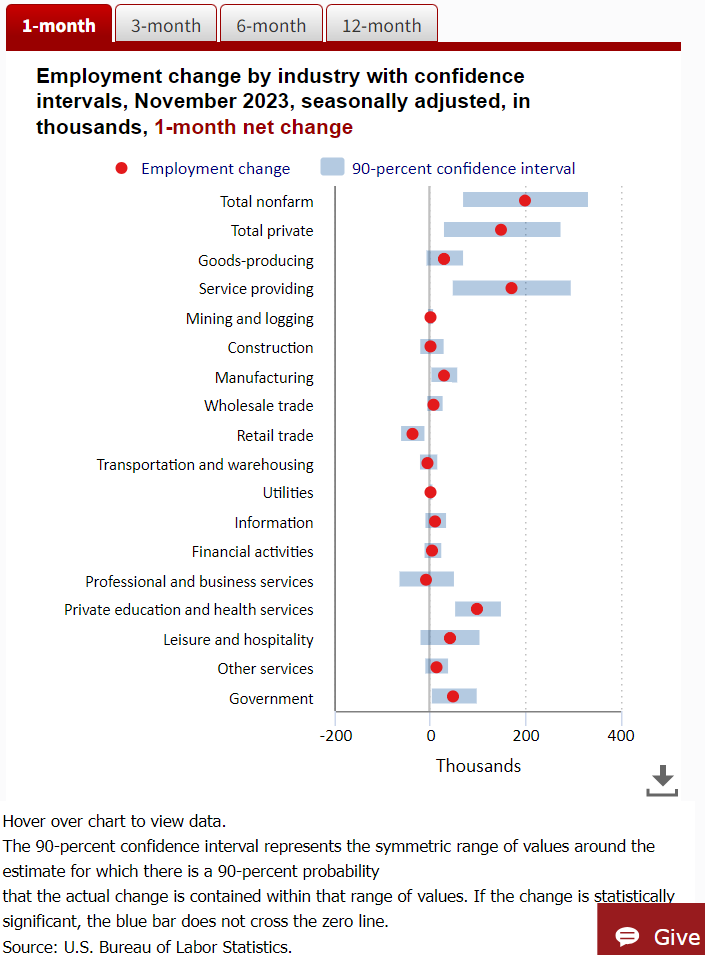
\includegraphics[width=0.4\textwidth,height=0.4\textheight]{const_emp.png}
\caption{Monthly Construction Employment}\label{fig:label}
}
\end{figure}

\begin{figure}
\hypertarget{fig:label}{%
\centering
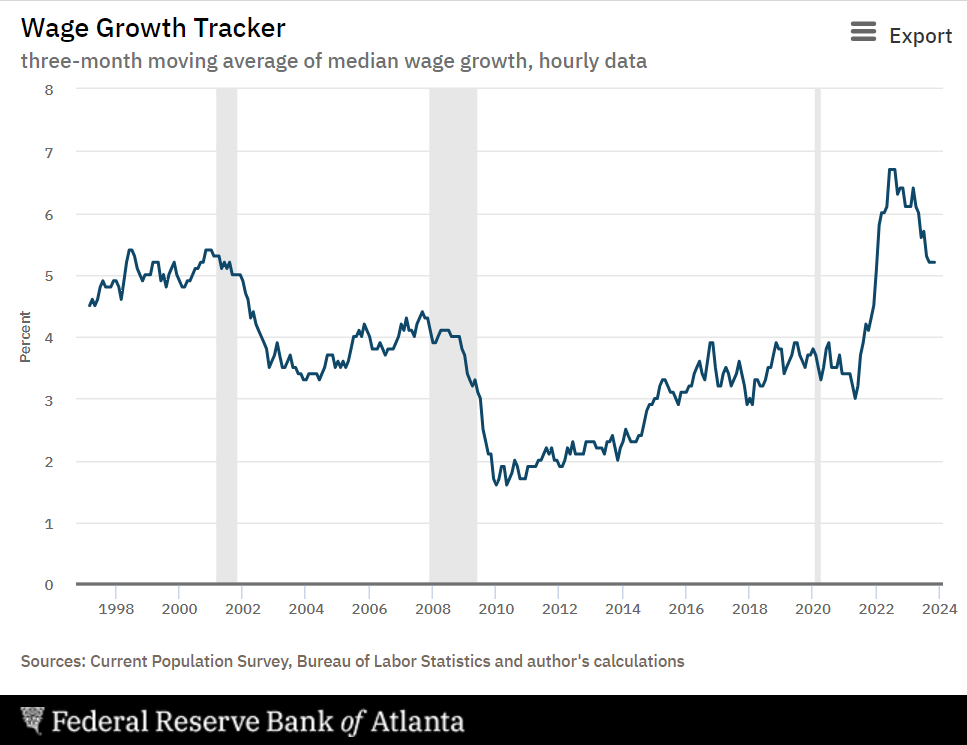
\includegraphics[width=0.4\textwidth,height=0.4\textheight]{const_wage.png}
\caption{Median Hourly Nominal Construction Wage}\label{fig:label}
}
\end{figure}

\begin{figure}
\hypertarget{fig:label}{%
\centering
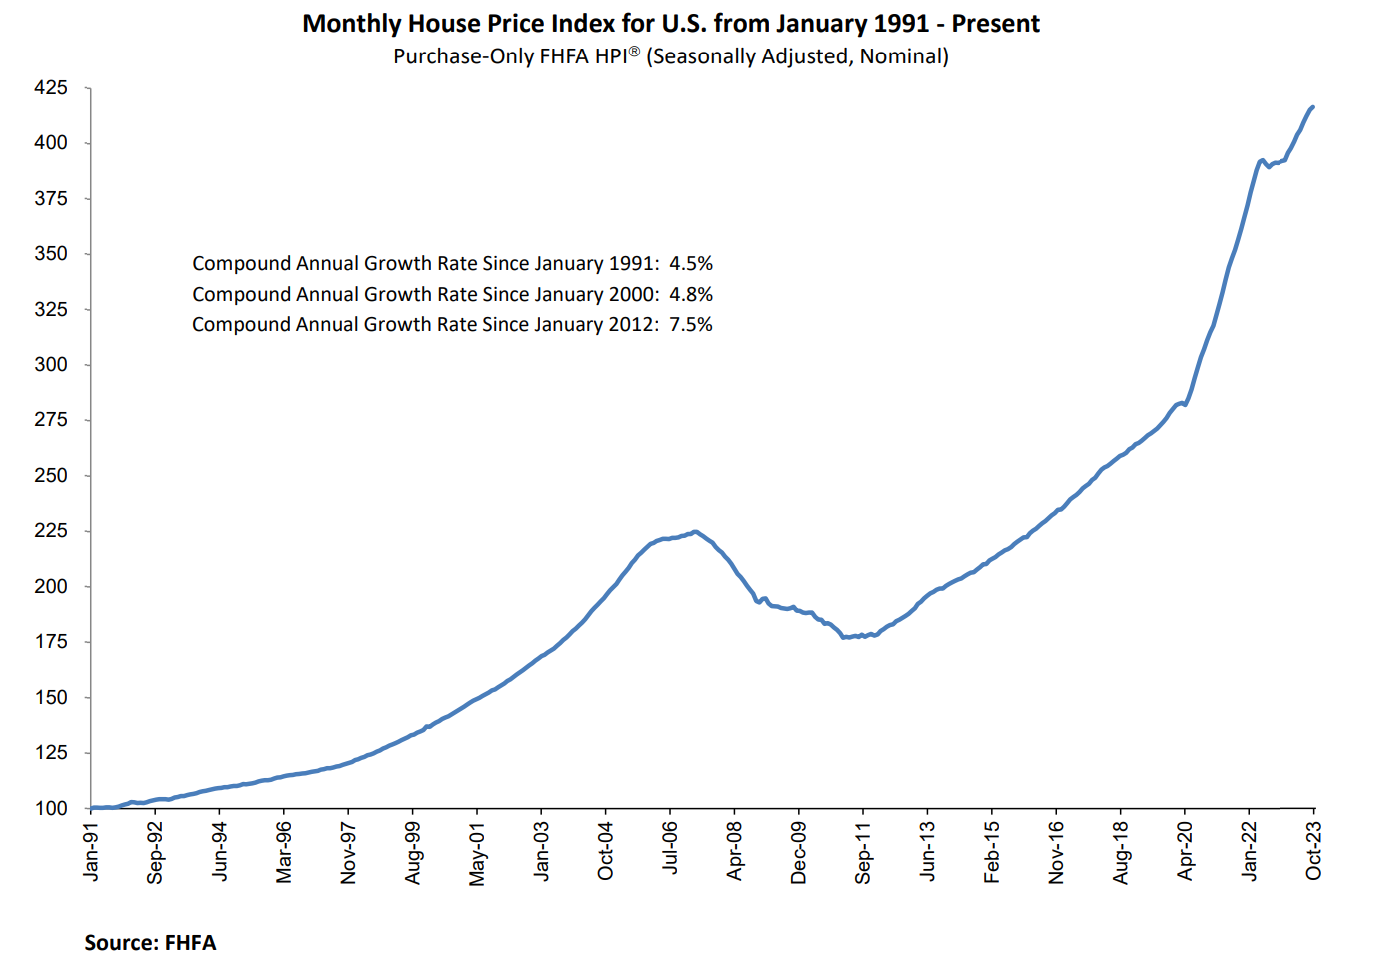
\includegraphics[width=0.4\textwidth,height=0.4\textheight]{fhfa_9123.png}
\caption{FHFA (Federal Housing Finance Agency) House Price
Index}\label{fig:label}
}
\end{figure}

\begin{figure}
\hypertarget{fig:label}{%
\centering
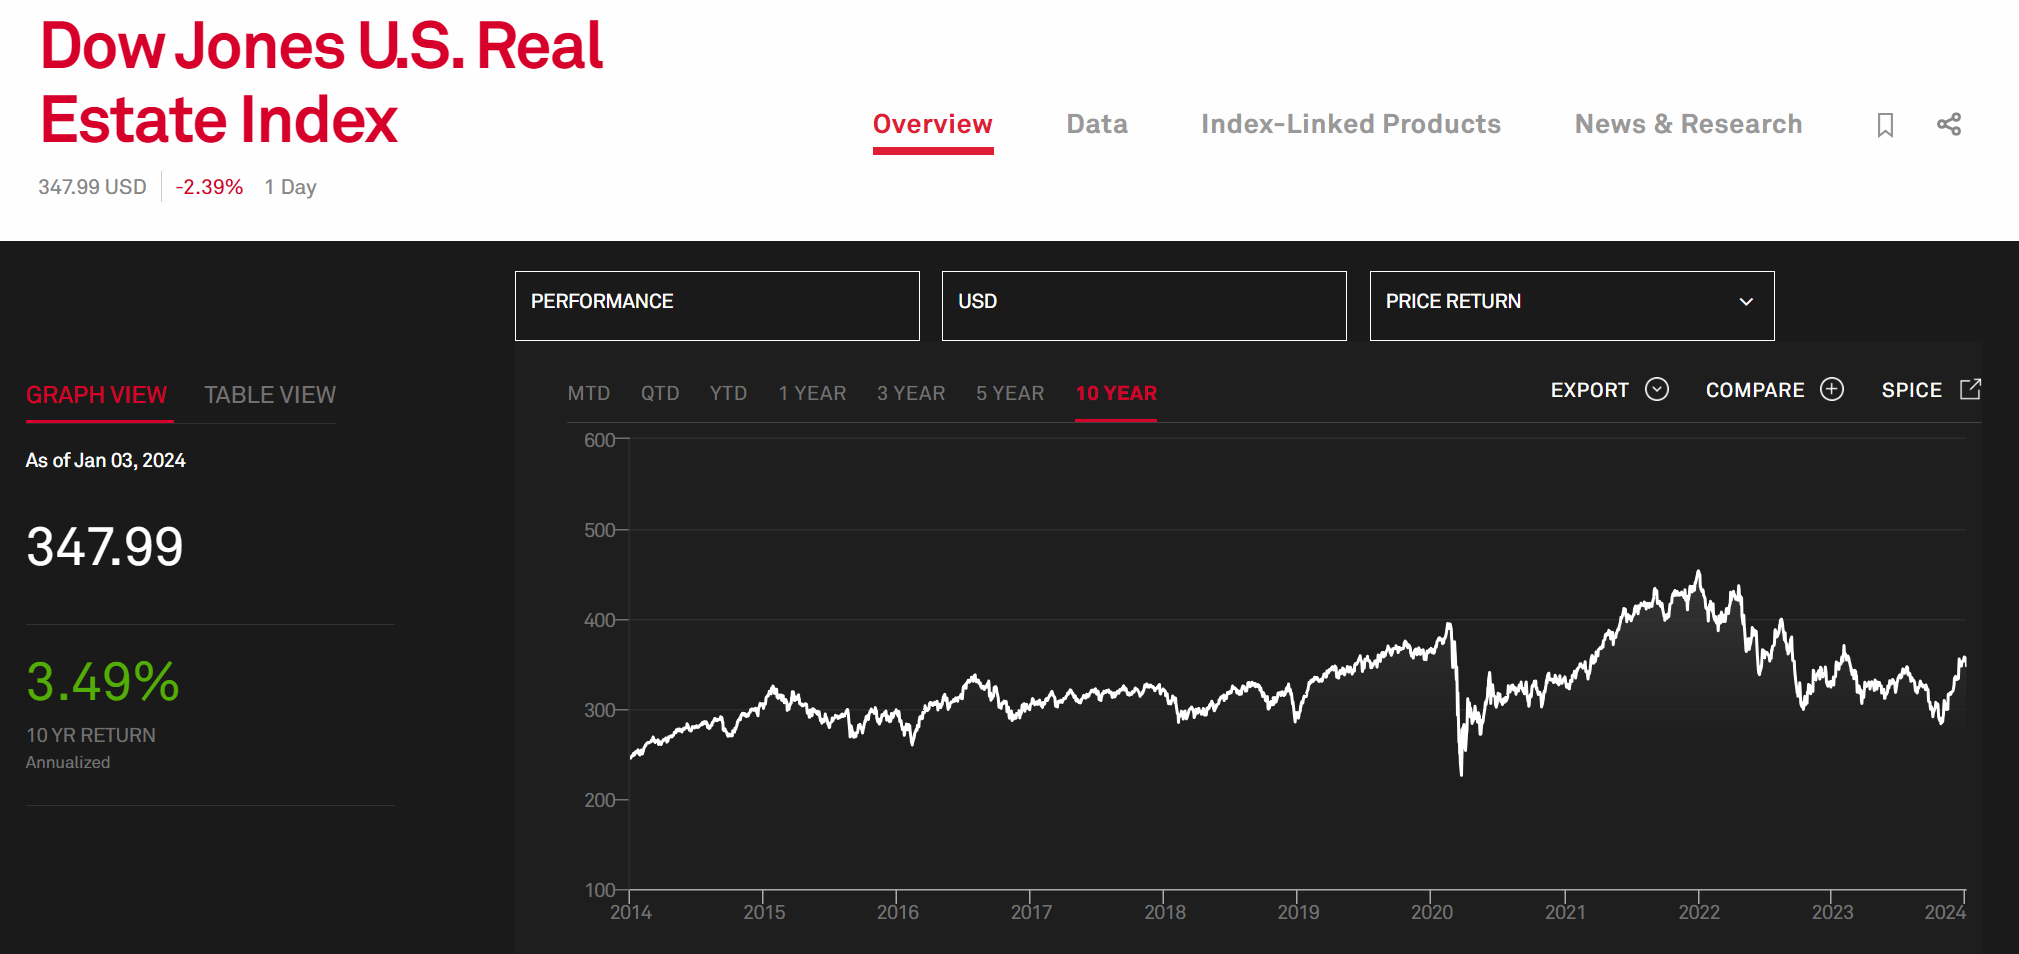
\includegraphics[width=0.4\textwidth,height=0.4\textheight]{djusrei_1423.png}
\caption{Dow Jones US Real Estate Index}\label{fig:label}
}
\end{figure}

\end{document}
